\documentclass[12pt, oneside]{article}

\usepackage[letterpaper, scale=0.8, centering]{geometry}
\usepackage{fancyhdr}
\setlength{\parindent}{0em}
\setlength{\parskip}{1em}

\pagestyle{fancy}
\fancyhf{}
\renewcommand{\headrulewidth}{0pt}
\rfoot{{\footnotesize Copyright Mia Minnes, 2022, Version \today~(\thepage)}}

\author{CSE105Sp22}

\newcommand{\instructions}{{\bf For all HW assignments:}

Weekly homework may be done individually or in groups of up to 3 students. 
You may switch HW partners for different HW assignments. 
The lowest HW score will not be included in your overall HW average. 
Please ensure your name(s) and PID(s) are clearly visible on the first page of your homework submission 
and then upload the PDF to Gradescope. If working in a group, submit only one submission per group: 
one partner uploads the submission through their Gradescope account and then adds the other group member(s) 
to the Gradescope submission by selecting their name(s) in the ``Add Group Members" dialog box. 
You will need to re-add your group member(s) every time you resubmit a new version of your assignment.
 Each homework question will be graded either for correctness (including clear and precise explanations and 
 justifications of all answers) or fair effort completeness. You may only collaborate on HW with CSE 105 students 
 in your group; if your group has questions about a HW problem, you may ask in drop-in help hours or post a private 
 post (visible only to the Instructors) on Piazza.

All submitted homework for this class must be typed. 
You can use a word processing editor if you like (Microsoft Word, Open Office, Notepad, Vim, Google Docs, etc.) 
but you might find it useful to take this opportunity to learn LaTeX. 
LaTeX is a markup language used widely in computer science and mathematics. 
The homework assignments are typed using LaTeX and you can use the source files 
as templates for typesetting your solutions.
To generate state diagrams of machines, we recommend using Flap.js
or JFLAP. Photographs of clearly hand-drawn diagrams may also be used. We recommend that you
submit early drafts to Gradescope so that in case of any technical difficulties, at least some of your
work is present. You may update your submission as many times as you'd like up to the deadline.


{\bf Integrity reminders}
\begin{itemize}
\item Problems should be solved together, not divided up between the partners. The homework is
designed to give you practice with the main concepts and techniques of the course, 
while getting to know and learn from your classmates.
\item You may not collaborate on homework with anyone other than your group members.
You may ask questions about the homework in office hours (of the instructor, TAs, and/or tutors) and 
on Piazza (as private notes viewable only to the Instructors).  
You \emph{cannot} use any online resources about the course content other than the class material 
from this quarter -- this is primarily to ensure that we all use consistent notation and
definitions we will use this quarter and also to protect the learning experience you will have when
the `aha' moments of solving the problem authentically happen.
\item Do not share written solutions or partial solutions for homework with 
other students in the class who are not in your group. Doing so would dilute their learning 
experience and detract from their success in the class.
\end{itemize}

}
\usepackage{amssymb,amsmath,pifont,amsfonts,comment,enumerate,enumitem}
\usepackage{currfile,xstring,hyperref,tabularx,graphicx,wasysym}
\usepackage[labelformat=empty]{caption}
\usepackage[dvipsnames,table]{xcolor}
\usepackage{multicol,multirow,array,listings,tabularx,lastpage,textcomp,booktabs}

\lstnewenvironment{algorithm}[1][] {   
    \lstset{ mathescape=true,
        frame=tB,
        numbers=left, 
        numberstyle=\tiny,
        basicstyle=\rmfamily\scriptsize, 
        keywordstyle=\color{black}\bfseries,
        keywords={,procedure, div, for, to, input, output, return, datatype, function, in, if, else, foreach, while, begin, end, }
        numbers=left,
        xleftmargin=.04\textwidth,
        #1
    }
}
{}
\lstnewenvironment{java}[1][]
{   
    \lstset{
        language=java,
        mathescape=true,
        frame=tB,
        numbers=left, 
        numberstyle=\tiny,
        basicstyle=\ttfamily\scriptsize, 
        keywordstyle=\color{black}\bfseries,
        keywords={, int, double, for, return, if, else, while, }
        numbers=left,
        xleftmargin=.04\textwidth,
        #1
    }
}
{}

\newcommand\abs[1]{\lvert~#1~\rvert}
\newcommand{\st}{\mid}

\newcommand{\A}[0]{\texttt{A}}
\newcommand{\C}[0]{\texttt{C}}
\newcommand{\G}[0]{\texttt{G}}
\newcommand{\U}[0]{\texttt{U}}

\newcommand{\cmark}{\ding{51}}
\newcommand{\xmark}{\ding{55}}
 
 
\title{HW2 : Regular Languages and Automata Constructions}
\date{Due: : 4/14/22 at 5pm (no penalty late submission until 8am next morning), via Gradescope}

\begin{document}
\maketitle
\thispagestyle{fancy}


{\bf In this assignment,}

You will practice designing multiple representations of regular languages
and working with general constructions of automata to demonstrate the 
richness of the class of regular languages.

{\bf Resources}: To review the topics you are working with 
for this assignment, see the class material from  Week 1 and the start of Week 2.
We will post frequently asked questions and our answers to them in a 
pinned Piazza post.

{\bf Reading and extra practice problems}: Sipser Section 1.1, 1.2, 1.3.
Chapter 1 exercises 1.4, 1.5, 1.6, 1.7, 1.8, 1.9, 1.10, 1.11, 1.12, 1.14, 1.15, 1.16, 1.17, 1.19, 1.20, 1.21, 1.22.

{\bf Key Concepts}: Regular expressions, language described by a regular expression, deterministic finite automata (DFAs), 
regular languages, closure of the class of regular languages under certain operations, 
nondeterministic finite automata (NFA).


\instructions

You will submit this assignment via Gradescope
(\href{https://www.gradescope.com}{https://www.gradescope.com}) 
in the assignment called ``HW2CSE105Sp22''.

{\bf Assigned questions}


\begin{enumerate}
\item ({\it Graded for correctness}\footnote{This means your solution will be
evaluated not only on the correctness of your answers, but on your ability to 
present your ideas clearly and logically. You should explain how you arrived at 
your conclusions, using 
mathematically sound reasoning. Whether you use formal proof techniques or 
write a more informal argument for why 
something is true, your answers should always be well-supported. Your goal 
should be to convince the reader that 
your results and methods are sound.}) Over the alphabet $\{a,b\}$, consider the language
\[
    L = \{ w \in \{a,b\}^* \mid (ab \textrm{ is a substring of $w$}) \land (ba \textrm{ is a substring of $w$})
    \land (w \textrm{ starts with } a)\}
\]
In this question, you will use two different approaches to proving that this language is 
regular by building (different) DFA that recognize this language.
\begin{enumerate}
    \item Design a DFA recognizing the language $\{ w \in \{a,b\}^* \mid ab \textrm{ is a substring of $w$}\}$
    and a DFA recognizing the language $\{ w \in \{a,b\}^* \mid ba \textrm{ is a substring of $w$}\}$
    and a third DFA recognizing the language $\{ w \in \{a,b\}^* \mid w \textrm{ starts with } a\}$. Then, 
    use the construction we discussed in class to combine these DFA to get a DFA that recognizes
    $L$. A complete solution will include the (clearly labelled) state diagrams for each 
    of the three building-block DFAs, along with a description of the result of combining these DFAs that includes
    the formal definition of the resulting DFA and 
    at the least the part of the state diagram that includes the start state, all the outgoing edges
    from the start state, and specifies
    how many states the full DFA will have.
    \item Rewrite the language $L$ in a simpler form and use this simpler form to design a DFA with at most
    $5$ states that recognizes $L$. A complete solution will include the complete state diagram 
    of this DFA and a justification for why the DFA recognizes $L$.
\end{enumerate}

\item  To safeguard the privacy or security of a network, some software filters
the IP addresses that are allowed to send content to computers on the network. Each IP address
can be broken into parts that represent the source host of incoming traffic, including geographic data.
As a result, software needs to be designed to recognize whether certain substrings (representing
permitted hosts) are present (if the hosts are permitted to send data) and whether others
are absent (if those hosts are blocked from sending data).

In this question, you'll design ways to detect these patterns in strings.

\begin{enumerate}
    \item ({\it Graded for correctness})
    Over the alphabet $\{0,1,2,3,4,5,6,7,8,9\}$ design a DFA that accepts each and only strings
    that have $384$ or $116$ as a substring. Your DFA should have {\bf no more than $8$ states}.
    A complete solution will include the state diagram of your DFA and a brief justification of
    your construction by explaining the role each state plays in the machine. {\it Note: you may 
    include the formal definition of your DFA, but this is not required.} 
    \item ({\it Graded for correctness})
    Now suppose the network administrators want to block traffic from IP addresses
    that have been associated with spammers. Over the alphabet~$\{0,1,2,3,4,5,6,7,8,9\}$, 
    design an NFA with at most $5$ states that accepts each and only strings
    that do not have the substring $384$ and do not have the substring $116$. 
    A complete solution will include the state diagram of your NFA and a brief justification 
    of your construction by explaining the role each state plays in the machine.
    \item ({\it Graded for fair effort completeness}\footnote{This means 
    you will get full credit so long as your submission demonstrates honest 
    effort to answer the question. You will not be penalized for incorrect answers. 
    To demonstrate your honest effort in answering the question, we ask that you 
    include your attempt to answer *each* part of the question. If you get stuck 
    with your attempt, you can still demonstrate your effort by explaining where 
    you got stuck and what you did to try to get unstuck.})
    Give a regular expression that describes the set of strings over 
    the alphabet $\{0,1,2,3,4,5,6,7,8,9\}$ that have $384$ as a substring and give
    a (different) regular expression that describes the set of strings over
    the alphabet $\{0,1,2,3,4,5,6,7,8,9\}$ that do not have $384$ as a substring. Briefly justify
    why each of your regular expression works.
\end{enumerate}

\item In this question, you'll practice working with formal general constructions
for DFAs and translating between state diagrams and formal definitions.
Consider the following
construction in the 
textbook for Chapter 1 Problem 34, which we include here for reference: 
``Let $B$ and $C$ be languages over $\Sigma = \{ 0,1\}$. Define
\[
B \overset{1}{\leftarrow} C= \{ w \in B ~\mid~\textrm{ for some $y \in C$, strings $w$ and $y$ contain equal 
numbers of $1$s }\}
\]
The class of regular languages is shown to be closed under the $\overset{1}{\leftarrow}$ operation
using the construction: Let $M_B = (Q_B, \Sigma, \delta_B, q_B, F_B)$ and $M_C = ( Q_C, \Sigma, \delta_C, q_C, F_C)$ be DFAs recognizing the languages $B$ and $C$, respectively.  We will now construct NFA
$M = (Q, \Sigma, \delta, q_0, F)$ that recognizes $B \overset{1}{\leftarrow} C$ as follows.  To decide
whether its input $w$ is in $B \overset{1}{\leftarrow} C$, the machine $M$ checks that $w \in B$, and 
in parallel nondeterministically guesses a string $y$ that contains the same number of $1$s as 
contained in $w$ and checks that $y \in C$.
\begin{itemize}
\item[{\bf 1.}] $Q = Q_B \times Q_C$
\item[{\bf 2.}] For $(q,r) \in Q$ and $a \in \Sigma_\varepsilon$, define
\[
\delta( ~((q,r), a)~) = \begin{cases}
\{ (\delta_B(q,0) , r ) \}  \qquad&\textrm{if } a = 0 \\
\{ (\delta_B( q,1) ,  \delta_C( r,1) ) \}  \qquad&\textrm{if } a = 1 \\
\{ (q, \delta_C( r,0 ))\}  \qquad&\textrm{if } a = \varepsilon\\
\end{cases}
\]
\item[{\bf 3.}] $q_0 = (q_B, q_C)$
\item[{\bf 4.}] $F = F_B \times F_C$~~~."
\end{itemize}

\begin{enumerate}
\item ({\it Graded for correctness}) Illustrate this construction by defining specific example DFAs $M_B$ and $M_C$ and including 
their state diagrams in your submission.   Choose $M_B$ to have four states and $M_C$
to have two states, and make sure that every state in each state diagram is reachable from the start state
of that machine.
Apply the construction above to create the NFA $M$  and include its state diagram in your submission.
{\it Note: you may 
 include the formal definition of your DFAs and NFA, but this is not required.} 

{\it Hint: Confirm that you have specified every required piece of the state diagram for $M$. E.g., 
label the states consistently with the construction, indicate the start arrow, specify each
accepting state, and include all required transitions.}

\item ({\it Graded for fair effort completeness})  Describe the sets recognized by each of the 
machines you used in part (a): $M_B, M_C, M$.
If possible, give an example of a string that is in $B$ and in $B \overset{1}{\leftarrow} C$
and an example of a string that is in $B$ and not in $B \overset{1}{\leftarrow} C$. If any of these examples
do not exist, explain why not.
\end{enumerate}


\item ({\it Graded for fair effort completeness}) In last week's homework, 
we saw the definitions of two functions on the set of languages over $\{0,1\}$:
for $L$ a set of strings over the alphabet $\{0,1\}$, we can define the following associated sets
\[
LZ(L) = \{ 0^k w \mid w \in L, k \in \mathbb{Z}, k \geq 0 \}
\]
\[
TZ(L) = \{ w 0^k \mid w \in L, k \in \mathbb{Z}, k \geq 0 \}
\]
In this question, we'll develop a general construction that will prove
that if $L$ is regular then so are $LZ(L)$ and $TZ(L)$.

Consider an arbitrary regular
language $L$ over the alphabet $\Sigma = \{0,1\}$, and we are given that
$M = (Q, \Sigma, \delta, q_0, F)$ is a DFA over $\Sigma$ with $L(M) = L$.

\begin{enumerate}
\item Give the formal construction of an NFA $M'$ with $L(M') = LZ(L)$.  Briefly justify 
each parameter in the definition of  $M'$.
\item Apply your construction from part (a) when $L_{test} = L(M_{test})$, where the 
state diagram $M_{test}$ is below.  Submit the state diagram of the NFA that results.
If possible, give an example of a string that is in $LZ(L_{test})$ and one that is not; if either of these examples
do not exist, explain why not.

\item Give the formal construction of an NFA $N'$ with $L(N') = TZ(L)$.  Briefly justify 
each parameter in the definition of  $N'$. 
\item Apply your construction from part (c)  when $L_{test} = L(M_{test})$, where the 
state diagram $M_{test}$ is below.  Submit the state diagram of the NFA that results.
If possible, give an example of a string that is in $TZ(L_{test})$ and one that is not; if either of these examples
do not exist, explain why not.
\begin{figure}[h]
   \centering
   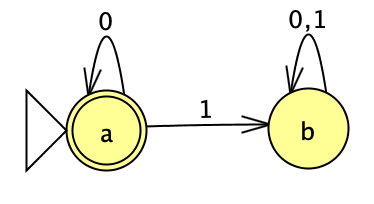
\includegraphics[width=2in]{MtestDFA.png}
   \caption{State diagram for DFA $M_{test}$}
\end{figure}
\end{enumerate}
{\it Caution}: Pay attention to the types of the components, especially
in the transition function.  You are given a DFA and are building an NFA.
\end{enumerate}
\end{document}